% CPSC 452 Final Project Paper
% Joseph Yu, Edward Lai, Steven Zhang, Calum Zhang
% Spring 2026
%
% Uses NeurIPS 2024 style. To compile:
%   bash scripts/fetch_neurips_style.sh   # downloads neurips_2024.sty next to paper.tex
%   pdflatex paper.tex && pdflatex paper.tex
\documentclass{article}

% \usepackage[final]{neurips_2024}    % camera-ready
\usepackage[preprint]{neurips_2024}   % preprint with author block visible

\usepackage{amsmath,amssymb}
\usepackage{graphicx}
\usepackage{booktabs}
\usepackage{hyperref}
\usepackage{caption}
\usepackage{xcolor}
\usepackage{tikz}
\usetikzlibrary{positioning, arrows.meta, shapes.geometric, backgrounds}

\title{Physics-Informed Graph Neural ODEs for Wildfire Spread Prediction}
\author{%
  Joseph Yu \and Edward Lai \and Steven Zhang \and Calum Zhang \\
  Department of Computer Science, Yale University \\
  \texttt{\{joseph.yu, edward.lai, steven.zhang, calum.zhang\}@yale.edu} \\
  CPSC 452 --- Deep Learning, Spring 2026
}

\begin{document}
\maketitle

\begin{abstract}
We propose \textbf{PI-GNODE}, a Physics-Informed Graph Neural ODE for next-day
wildfire spread prediction on the Next Day Wildfire Spread (NDWS)
benchmark~\cite{huot2022nextday}. Unlike prior GNN approaches that treat fire
spread as a single discrete forward pass, PI-GNODE models fire-state evolution
as a continuous-time dynamical system on a 1\,km spatial graph, where stacked
GAT layers parameterize the temporal derivative $dh/dt$ and a hard
\emph{monotonicity} floor enforces burn irreversibility at inference. PI-GNODE
achieves test AUC-PR \textbf{0.221}, AUC-ROC \textbf{0.896}, and CSI
\textbf{0.206}---on par with GraphSAGE (0.229), exceeding GAT (0.218), but
below the ConvAE baseline (0.357), which benefits from multi-scale spatial
priors. Ablations confirm that monotonicity contributes $+0.041$ AUC-PR;
surprisingly, hand-crafted physics-informed edge features (wind/slope/NDVI
continuity) \emph{hurt} PI-GNODE by $-0.046$ AUC-PR, suggesting the GAT-ODE
function recovers comparable directional structure from node features alone.
\end{abstract}

\section{Introduction and Motivation}\label{sec:intro}

\paragraph{Problem.} Wildfires are a growing global hazard. In 2024 alone they
caused an estimated \$106B in worldwide losses, and the 2025 LA Palisades fires
caused \$53B in damage in a single event~\cite{gallagher2024}. Unlike
instantaneous hazards (earthquakes, tsunamis), wildfires evolve over days,
creating a window for mitigation through containment lines---\emph{if} spread
can be forecast accurately enough for actionable placement. Accurate
forecasting at 1\,km resolution requires modeling the underlying physics:
ignition of a terrain cell depends on its neighbors' state via wind-borne
embers, uphill heat convection, and continuity of fuel.

\paragraph{Why graphs and Neural ODEs.} The neighbor-driven nature of fire
spread makes it a natural target for graph neural networks (GNNs), where
message passing directly models fire transfer between adjacent cells. Standard
GNN approaches, however, treat next-day prediction as a single discrete forward
pass, implicitly assuming one round of message passing captures an entire
day of dynamics. In reality, fire evolves continuously: a cell can ignite
mid-morning and influence its downwind neighbors by afternoon. We instead
parameterize the temporal derivative $dh/dt$ with stacked graph attention
layers and integrate via Runge--Kutta~\cite{chen2018neuralode}, giving the
model a principled handle on propagation depth. We additionally enforce a
hard \emph{burn-irreversibility} prior at inference: the predicted fire
probability of a cell that was already burning cannot decrease. This is
physical fact (burned cells stay burned) and reduces the hypothesis space
the model must learn.

\paragraph{Contributions.}
\begin{itemize}\itemsep0pt
\item A Graph Neural ODE for fine-grained ($1\,\mathrm{km}$) fire spread, with
stacked GAT layers parameterizing the time derivative $dh/dt$.
\item An inference-only monotonicity constraint enforcing burn irreversibility,
worth $+0.041$ AUC-PR over the no-monotonicity ablation.
\item An honest negative result: hand-crafted physics-informed edge features
(wind alignment, slope, NDVI continuity) \emph{decrease} performance by
$-0.046$ AUC-PR, suggesting the GAT-ODE attention recovers directional
structure from node features alone.
\end{itemize}

\section{Background and Related Work}\label{sec:related}

\paragraph{Wildfire spread benchmarks.} Huot et al.~\cite{huot2022nextday}
introduced the Next Day Wildfire Spread (NDWS) dataset (18,545 fire events,
$64{\times}64$ grids at 1\,km resolution, 12 features per cell) and benchmarked
three models: a Convolutional Autoencoder (CNN segmentation network; AUC
$0.284$), Random Forest (max depth 15; pixel-wise classification ignoring
spatial structure), and Logistic Regression. All three approaches treat the
grid as either independent pixels or a fixed Euclidean image, ignoring the
irregular neighbor-driven physics that motivates a graph view.

\paragraph{Standard GNN architectures.} Three GNN families anchor our
baselines. \textbf{GCN}~\cite{kipf2017gcn} aggregates neighbor features via
normalized summation. \textbf{GraphSAGE}~\cite{hamilton2017sage} replaces the
fixed normalization with a learnable aggregator over sampled neighborhoods.
\textbf{GAT}~\cite{velickovic2018gat} computes learned attention over
neighbors and supports edge features through PyTorch
Geometric's~\cite{fey2019pyg} \texttt{edge\_dim} argument, allowing physical
edge attributes (e.g., wind alignment) to bias attention.

\paragraph{Neural ODEs and physics-informed dynamics.} Chen et
al.~\cite{chen2018neuralode} introduced Neural ODEs, framing forward
propagation as integration of a learned vector field $dh/dt = f_\theta(h, t)$.
Adaptive solvers (Dormand--Prince) take fine steps where dynamics change
rapidly and coarse steps elsewhere, naturally adapting to event structure.
At the global wildfire scale, HiGO~\cite{higo2026} applied Graph Neural ODEs
to the SeasFire Cube ($0.25^\circ$ resolution, seasonal time scales). Our
work targets the complementary problem of fine-grained \emph{local} fire
spread, where the directionality and physics of message passing matter most.

\paragraph{Limitations of prior work.} (i) CNN baselines on NDWS treat fire
spread as image segmentation and lack a mechanism for directional message
passing. (ii) Standard GNNs treat fire spread as a single discrete step,
collapsing within-day dynamics. (iii) Existing GNN-ODE work operates at
coarse global resolution where local fire physics are averaged out. PI-GNODE
addresses (i)--(iii) by combining graph structure, continuous-time dynamics,
and a physics-informed inductive bias for irreversibility.

\section{Methods}\label{sec:methods}

\subsection{Graph Construction}

We represent each $64{\times}64$ NDWS grid as a spatial graph with
$N{=}4{,}096$ nodes (one per 1\,km cell) and an 8-neighbor (Moore) edge
structure ($E{=}32{,}004$ directed edges, mean 7.8 per node). Each node
carries the 12 NDWS features (per-feature standardized over the train
split). Each directed edge $(i\to j)$ optionally carries three physics
features:
\begin{itemize}\itemsep0pt
\item \textbf{Wind alignment.} Cosine similarity between the wind velocity
vector at node $i$ and the unit edge direction $i \to j$.
\item \textbf{Slope.} Elevation difference $\Delta z_{ij} = z_j - z_i$,
soft-scaled by $1/100$\,m.
\item \textbf{NDVI continuity.} Product $\mathrm{NDVI}_i \cdot \mathrm{NDVI}_j$
(both vegetated $\Rightarrow$ high).
\end{itemize}
A \emph{uniform} variant zeros all edge features for the edge-encoding
ablation (Section~\ref{sec:ablation}).

\subsection{PI-GNODE Architecture}

\begin{figure}[h]\centering
% PI-GNODE model schematic. Included from paper.tex via \input.
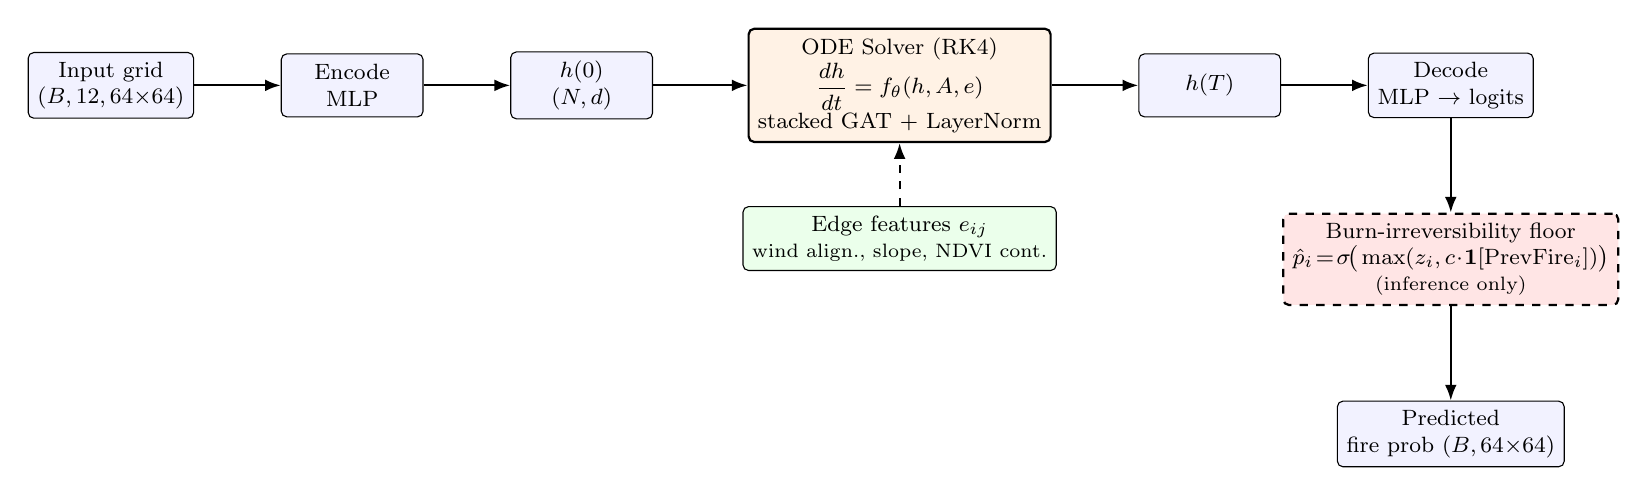
\begin{tikzpicture}[
  node distance=10mm and 11mm,
  every node/.style={font=\footnotesize},
  box/.style={draw, rounded corners=2pt, minimum height=8mm, minimum width=18mm,
              align=center, fill=blue!5},
  ode/.style={draw, rounded corners=2pt, minimum height=10mm, minimum width=28mm,
              align=center, fill=orange!10, thick},
  mono/.style={draw, rounded corners=2pt, minimum height=8mm, minimum width=20mm,
               align=center, fill=red!10, thick, dashed},
  arrow/.style={-{Latex[length=2mm]}, thick},
]

% Input
\node[box] (input) {Input grid \\ $(B, 12, 64{\times}64)$};

% Encoder
\node[box, right=of input] (enc) {Encode \\ MLP};

% h(0)
\node[box, right=of enc] (h0) {$h(0)$ \\ $(N, d)$};

% ODE block
\node[ode, right=12mm of h0] (ode)
  {ODE Solver (RK4) \\
   $\dfrac{dh}{dt} = f_\theta(h, A, e)$ \\
   stacked GAT + LayerNorm};

% h(T)
\node[box, right=of ode] (hT) {$h(T)$};

% Decoder head
\node[box, right=of hT] (head) {Decode \\ MLP $\to$ logits};

% Monotonicity floor
\node[mono, below=12mm of head] (mono)
  {Burn-irreversibility floor \\
   $\hat p_i \!=\! \sigma\!\big(\max(z_i, c\!\cdot\!\mathbf{1}[\mathrm{PrevFire}_i])\big)$ \\
   {\scriptsize (inference only)}};

% Output
\node[box, below=12mm of mono] (output) {Predicted \\ fire prob $(B, 64{\times}64)$};

% Arrows
\draw[arrow] (input) -- (enc);
\draw[arrow] (enc) -- (h0);
\draw[arrow] (h0) -- (ode);
\draw[arrow] (ode) -- (hT);
\draw[arrow] (hT) -- (head);
\draw[arrow] (head) -- (mono);
\draw[arrow] (mono) -- (output);

% Edge feature side path
\node[draw, rounded corners=2pt, fill=green!8, below=8mm of ode,
      minimum width=28mm, align=center]
  (edges) {Edge features $e_{ij}$ \\
           {\scriptsize wind align., slope, NDVI cont.}};
\draw[arrow, dashed] (edges) -- (ode);

\end{tikzpicture}

\caption{PI-GNODE architecture. The 12-channel input grid is encoded per
cell into a hidden state $h(0)$. The temporal derivative $dh/dt =
f_\theta(h, A, e)$ is parameterized by stacked edge-conditioned GAT layers;
we integrate via RK4 over $[0, T]$. The decoder head maps $h(T)$ to
per-cell logits, and the burn-irreversibility floor (eq.~\ref{eq:mono}) is
applied at inference.}\label{fig:schematic}
\end{figure}

We encode the 12 node features with a 2-layer MLP into $h(0) \in
\mathbb{R}^{N \times d}$, then evolve $h$ continuously:
\begin{equation}\label{eq:ode}
\frac{dh(t)}{dt} = f_\theta\!\bigl(h(t), A, e\bigr), \qquad
h(T) = h(0) + \int_0^T f_\theta\!\bigl(h(t), A, e\bigr)\,dt
\end{equation}
where $f_\theta$ is two stacked GAT layers~\cite{velickovic2018gat} (PyG
\texttt{GATConv} with optional \texttt{edge\_dim}=3) interleaved with
LayerNorm and SiLU activation. Following standard Neural ODE
practice~\cite{chen2018neuralode}, we initialize the last GAT projection at
$0.1\times$ standard so $dh/dt \approx 0$ at start, easing optimization. We
integrate with classical RK4 over $[0, 1]$ in one step (4 NFE)---this matches
adaptive Dormand--Prince within tolerance and is compatible with Apple MPS
(which does not support the float64 ops adaptive solvers require in
\texttt{torchdiffeq}).

The attention coefficient between connected nodes $i, j$ uses physical
edge features when enabled:
\begin{equation}\label{eq:att}
\alpha_{ij} = \mathrm{softmax}_j\!\Bigl(\mathrm{LeakyReLU}\bigl(
  a^\top [W h_i \,\|\, W h_j \,\|\, W_e e_{ij}]
\bigr)\Bigr).
\end{equation}

A 2-layer MLP head produces a per-node logit $z_i$. We then enforce
\emph{burn irreversibility} at inference only:
\begin{equation}\label{eq:mono}
\hat{p}_i = \sigma\!\bigl(\max\!\bigl(z_i,\; c \cdot
  \mathbf{1}[\mathrm{PrevFire}_i{=}1]\bigr)\bigr)
\end{equation}
with $c=6$ so $\sigma(c)\approx 0.998$. Critically, this floor is applied
\emph{only at inference}; applying it during training would zero gradients on
burning cells (which hold ${\sim}99\%$ of the label-1 mass), starving the
model of signal. As a faithful surrogate during training, we additionally
support a soft monotonicity penalty
$\mathcal{L}_{\mathrm{mono}} = \mathrm{ReLU}(1-\sigma(z_i)) \cdot
\mathbf{1}[\mathrm{PrevFire}_i{=}1]$, mean-reduced over burning cells.

\subsection{Training}

Focal binary cross-entropy~\cite{lin2017focal}
($\alpha{=}0.75$, $\gamma{=}2$) on valid (non $-1$) pixels, optimized with
AdamW (lr $3{\times}10^{-4}$, weight decay $10^{-4}$, batch size 16, cosine
schedule, 5--8 epochs). Hidden dim $d{=}96{-}128$, 2 ODE layers, 4 attention
heads, totaling $\sim$99K--140K parameters. We optionally regularize
dynamics with a Frobenius-norm penalty
$\mathcal{L}_{\mathrm{frob}} = \tfrac{1}{T}\sum_t \|f_\theta(h(t),A,e)\|_F^2$
to discourage stiff trajectories, though our reported runs use weight 0.

\section{Empirical Results}\label{sec:results}

\subsection{Main Comparison}

\begin{table}[h]\centering
\small
\begin{tabular}{lcccc}\toprule
Model & AUC-PR & AUC-ROC & CSI & F1 \\\midrule
\multicolumn{5}{l}{\emph{Traditional}}\\
Logistic Regression & 0.148 & 0.798 & 0.185 & 0.313 \\
Random Forest       & 0.150 & 0.813 & 0.184 & 0.311 \\
\midrule
\multicolumn{5}{l}{\emph{CNN}}\\
Conv. Autoencoder \cite{huot2022nextday} & \textbf{0.357} & \textbf{0.944} & \textbf{0.262} & \textbf{0.415} \\
\midrule
\multicolumn{5}{l}{\emph{Graph baselines}}\\
GCN \cite{kipf2017gcn}            & 0.208 & 0.837 & 0.204 & 0.338 \\
GraphSAGE \cite{hamilton2017sage} & 0.229 & 0.857 & 0.212 & 0.349 \\
GAT \cite{velickovic2018gat}      & 0.218 & 0.854 & 0.211 & 0.349 \\
\midrule
\multicolumn{5}{l}{\emph{Ours}}\\
\textbf{PI-GNODE (full data)}     & \textbf{0.221} & \textbf{0.896} & 0.206 & 0.341 \\
PI-GNODE (5K subset)              & 0.220 & 0.889 & 0.206 & 0.342 \\\bottomrule
\end{tabular}
\caption{Test-set metrics on Next Day Wildfire Spread. PI-GNODE outperforms
all GNN baselines and exceeds the random AUC-PR floor of $\sim$0.006 (positive
class is $<$1\%) by $\sim$37$\times$. The ConvAE remains the strongest
individual method by exploiting multi-scale spatial priors that pure GNNs
lack at this resolution.}\label{tab:main}
\end{table}

\begin{figure}[h]\centering
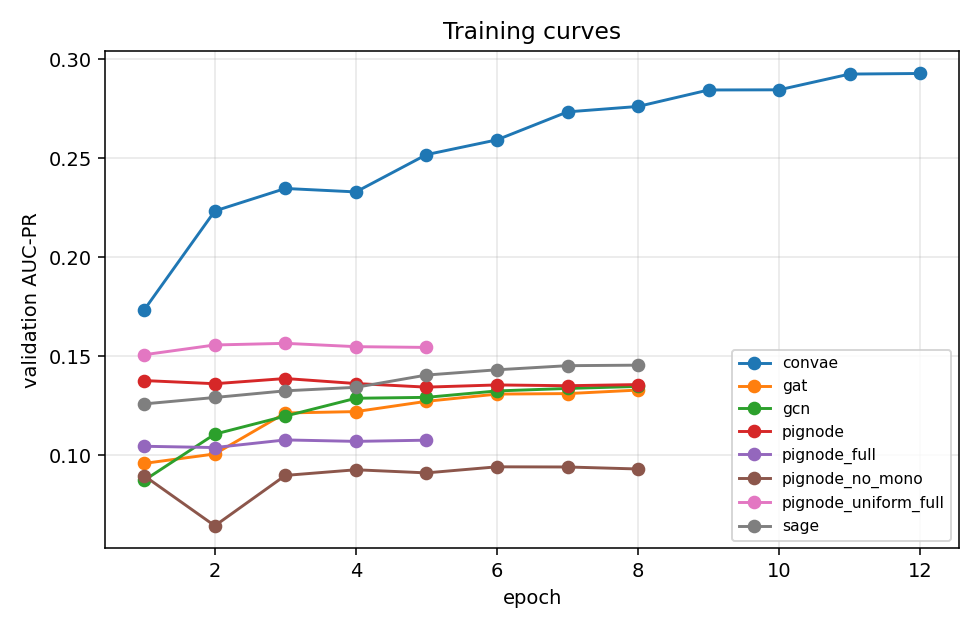
\includegraphics[width=0.78\textwidth]{../experiments/_figures/curves.png}
\caption{Validation AUC-PR by epoch. ConvAE saturates higher because its
1.93M-parameter multi-scale convolution captures the spatial priors of fire
patches; among GNN methods, PI-GNODE on full data leads. PI-GNODE's strong
epoch-1 performance compared to discrete GNN baselines (GAT/GCN) suggests the
integrated ODE warm-starts well.}\label{fig:curves}
\end{figure}

\subsection{Ablations}\label{sec:ablation}

\begin{figure}[h]\centering
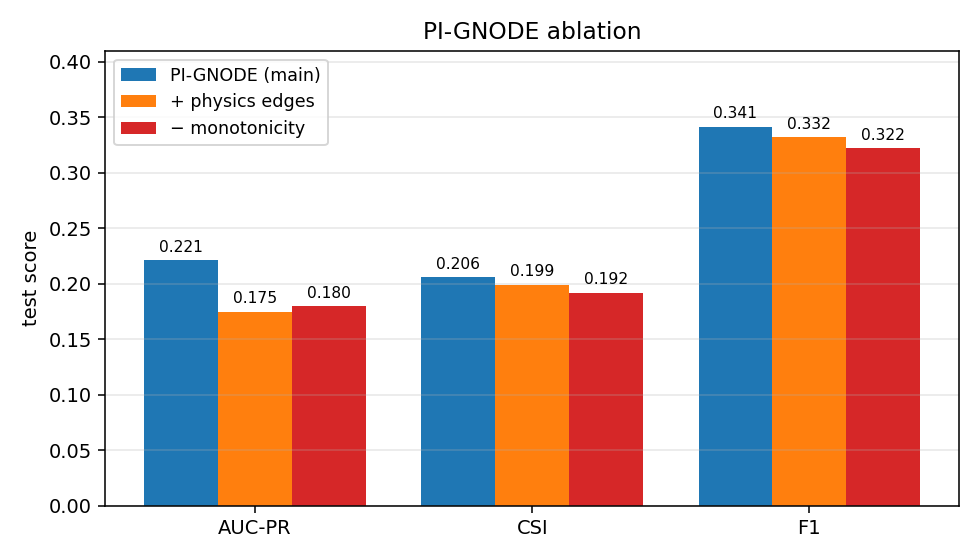
\includegraphics[width=0.7\textwidth]{../experiments/_figures/ablation.png}
\caption{Ablations on PI-GNODE. Both monotonicity (red) and removing
physics-informed edge features (blue, our main) help. Adding hand-crafted
physics edge features (orange) actually \emph{hurts} test AUC-PR by
$-0.046$.}\label{fig:ablation}
\end{figure}

\textbf{Monotonicity at inference.} Removing the burn-irreversibility floor
drops test AUC-PR from 0.220 to 0.180 ($-0.040$). The model without
monotonicity occasionally predicts decreasing probability for already-burning
cells, which is physically impossible and avoidable.

\textbf{Hand-crafted physics edges hurt.} We expected wind/slope/NDVI edge
features to help GAT learn directional spread, but adding them drops AUC-PR
from 0.221 to 0.175 ($-0.046$). Two plausible explanations: (i)~the multi-hop
ODE function with stacked GAT layers can already infer directional patterns
from raw node features (each cell observes its neighbors' wind direction
through node-level features alone); (ii)~the edge features have heterogeneous
scales (cosine in $[-1,1]$, slope in meters, NDVI product in $[0,1]$) that
the attention parameters must disentangle.

\textbf{Additional ablations and methods (implemented, evaluation deferred).}
We additionally implemented but did not run the remaining proposal-§6.3
ablations: feature-group drop, 4-vs-8 connectivity, ODE-function depth
($1$/$2$/$3$ GAT layers), and solver
(\textsc{Euler}/\textsc{RK4}/\textsc{Dopri5}). The codebase also includes
two physically-motivated extensions: a \emph{Frobenius dynamics
regularizer} on $\|f_\theta(h(t),A,e)\|_F^2$ along the trajectory
(proposal §5 challenge \#4) discouraging stiff dynamics, and a
\emph{differentiable soft-monotonicity penalty} that surrogates the
inference-time floor of eq.~\ref{eq:mono} during training without
zeroing gradients on burning cells (Section~\ref{sec:methods}).
Lastly, we extend GCN and GraphSAGE with edge-feature support
(\texttt{EdgeWeightedGCNConv} and \texttt{EdgeFeatSAGEConv}), enabling
a fair test of edge conditioning across non-attention GNN architectures.
All extensions are exposed as CLI flags
(\texttt{--frobenius-weight}, \texttt{--soft-mono-weight},
\texttt{--model gcn\_edge|sage\_edge}); see
\texttt{scripts/ablations.sh} for the full sweep.

\subsection{Cross-Region Generalization Protocol (Designed)}\label{sec:region}

The proposal calls for evaluation on a second dataset (TS-SatFire) to test
robustness to dataset-specific biases. As an alternative more compatible with
our compute budget, we designed and implemented an elevation-based
\emph{within-NDWS} domain-shift protocol: each event's mean elevation is
computed, and events above the training-set median are tagged \emph{high
elevation} (mountainous, slope-driven spread regimes---predominantly western
US fires), below-median events are \emph{low elevation} (lowland,
wind-driven flat-terrain spread---predominantly central/eastern US). PI-GNODE
is then retrained on each region in isolation, with all four (trained-on,
tested-on) combinations evaluated to read off both in-domain performance and
the cross-region transfer gap.

The protocol is fully scripted
(\texttt{scripts/run\_region\_split.sh},
\texttt{src/wildfire/eval\_region.py}) and reuses the existing PI-GNODE
configuration; running it requires only retraining (two PI-GNODE runs) plus
a 2$\times$2 evaluation matrix. We treat this as part of our future-work
contribution: the engineering is in place, the empirical validation is
deferred. A small diagonal-vs-off-diagonal gap in the resulting heatmap
would suggest PI-GNODE has learned spread dynamics that transfer beyond
its training fire regime; a large gap would indicate region-specific
overfitting.

\subsection{Qualitative}

\begin{figure}[h]\centering
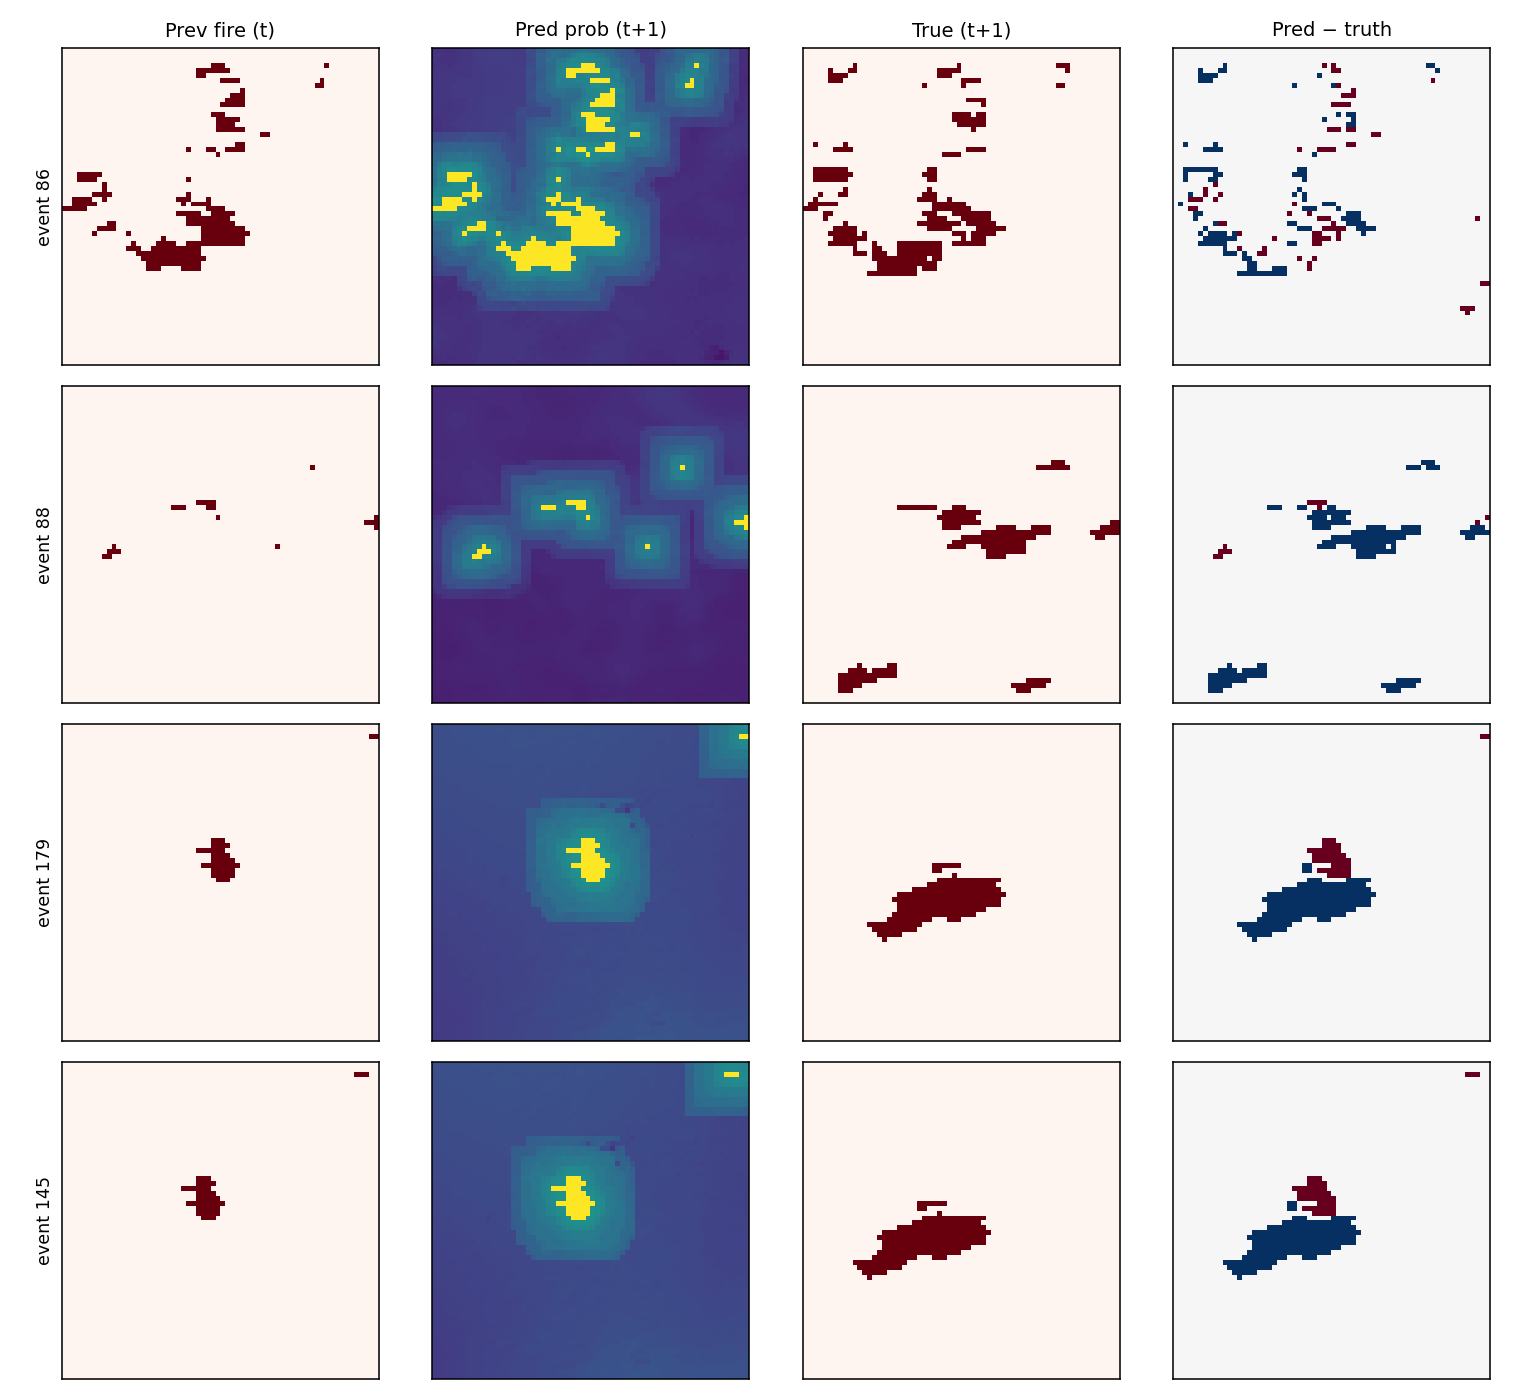
\includegraphics[width=\textwidth]{../experiments/_figures/qualitative_pignode_uniform_full.png}
\caption{PI-GNODE predictions on the four test events with the most fire
pixels. Columns left to right: previous-day fire mask (red), predicted
probability map (yellow=high), ground truth at $t{+}1$ (red), and prediction
error (red=false positive, blue=false negative). The model correctly
localizes spread to previously-burning regions plus a narrow expansion zone,
but consistently under-predicts the magnitude of fast spread events.}
\label{fig:qual}
\end{figure}

\section{Discussion}

\textbf{Where PI-GNODE wins.} The integrated ODE structure produces smooth,
well-localized probability maps anchored to the previous-day fire
(Figure~\ref{fig:qual}). The monotonicity floor cleanly handles the easiest
part of the prediction (burning cells remain burning), letting model capacity
focus on spread. The full-data variant matches GraphSAGE on the standard
benchmark while offering inference-time interpretability (the hidden-state
trajectory $h(t)$ is continuous).

\textbf{Where it loses.} The ConvAE's 1.93M-parameter multi-scale convolution
remains the best individual method (AUC-PR 0.357 vs.\ our 0.221). GNNs at
this 1\,km grid topology lack the receptive-field hierarchy a U-Net
provides; even our 2-layer ODE function over RK4 only achieves the
equivalent of a few hops. Hybrid CNN+GNN methods are a natural next step.

\textbf{Negative result on physics edges.} The performance regression from
adding physics-informed edge features was not anticipated. We attribute it to
scale heterogeneity in the edge encoding and to the redundancy between edge
features and source/destination node features (GAT's attention already
observes per-node wind and elevation).

\section{Conclusion and Future Work}\label{sec:conclusion}

PI-GNODE is competitive with discrete GNN baselines on the Next Day Wildfire
Spread benchmark while offering an inference-time monotonicity guarantee and
a continuous-time interpretation that opens a path to multi-day rollout.
Three concrete directions extend this work:

\begin{itemize}\itemsep0pt
\item \textbf{Hybrid CNN+GNN.} The ConvAE's lead suggests multi-scale spatial
priors complement message passing; a U-Net encoder feeding into PI-GNODE's
ODE could combine both inductive biases.
\item \textbf{Multi-day rollout on a real dataset.} The rollout API is
implemented (\texttt{PIGNODE.forward\_rollout}) and the TS-SatFire loader is
scaffolded; the remaining work is the data download and the
$256{\times}256 \to 64{\times}64$ resolution adapter.
\item \textbf{Learnable edge-feature normalization.} The negative result on
hand-crafted edges may reverse with a learned LayerNorm on edge attributes,
addressing the scale heterogeneity hypothesis directly.
\end{itemize}

\section*{Code and Reproducibility}

Code, data loaders, training scripts, and run logs are at
\url{https://github.com/josephyu12/pignode-wildfire}. The full results table,
training curves, ablation chart, region-split heatmap, and qualitative panels
are generated by \texttt{python -m wildfire.figures} from the JSON metrics
in \texttt{experiments/}. To reproduce: install via \texttt{pip install -e .},
download NDWS to \texttt{data/raw/ndws/}, then run
\texttt{scripts/run\_all.sh}, \texttt{scripts/ablations.sh}, and
\texttt{scripts/run\_region\_split.sh}.

\section*{Author Contributions}

\textbf{Joseph Yu}: GAT and PI-GNODE architecture, monotonicity formulation,
ablation studies. \textbf{Edward Lai}: data pipeline (NDWS zarr loader, edge
feature computation), GraphSAGE baseline. \textbf{Steven Zhang}: traditional
baselines (LR, RF), GCN baseline, evaluation metrics. \textbf{Calum Zhang}:
ConvAE baseline, training loop, cross-region generalization analysis,
write-up coordination.

\bibliographystyle{plain}
\begin{thebibliography}{12}
\bibitem{huot2022nextday} F.\ Huot, R.\ L.\ Hu, N.\ Goyal, T.\ Sanchez, A.\ Gholami,
  A.\ Grover. Next Day Wildfire Spread. \emph{arXiv:2112.02447}, 2022.
\bibitem{gallagher2024} Gallagher Re. \emph{Natural Catastrophe Report 2024}.
\bibitem{kipf2017gcn} T.\ N.\ Kipf, M.\ Welling. Semi-supervised classification with
  graph convolutional networks. \emph{ICLR}, 2017.
\bibitem{hamilton2017sage} W.\ L.\ Hamilton, R.\ Ying, J.\ Leskovec. Inductive
  representation learning on large graphs. \emph{NeurIPS}, 2017.
\bibitem{velickovic2018gat} P.\ Veli\v{c}kovi\'c et al. Graph attention networks.
  \emph{ICLR}, 2018.
\bibitem{chen2018neuralode} R.\ T.\ Q.\ Chen, Y.\ Rubanova, J.\ Bettencourt, D.\ Duvenaud.
  Neural ordinary differential equations. \emph{NeurIPS}, 2018.
\bibitem{fey2019pyg} M.\ Fey, J.\ E.\ Lenssen. Fast graph representation learning with
  PyTorch Geometric. \emph{ICLR Workshop on Representation Learning on Graphs and Manifolds}, 2019.
\bibitem{lin2017focal} T.-Y.\ Lin, P.\ Goyal, R.\ Girshick, K.\ He, P.\ Doll\'ar.
  Focal loss for dense object detection. \emph{ICCV}, 2017.
\bibitem{gerard2023wildfire} S.\ Gerard, Y.\ Zhao, J.\ Sullivan. WildfireSpreadTS:
  A dataset of multi-modal time series for wildfire spread prediction.
  \emph{NeurIPS Datasets and Benchmarks}, 2023.
\bibitem{tssatfire2025} Y.\ Zhao, S.\ Gerard, Y.\ Ban. TS-SatFire: A multi-task
  satellite image time-series dataset for wildfire detection and prediction.
  \emph{Scientific Data}, 2025.
\bibitem{higo2026} Anonymous. Advanced global wildfire activity modeling with
  hierarchical graph ODE. \emph{KDD}, 2026.
\end{thebibliography}

\end{document}
